% Лабораторная работа по Системному Программированию № 2
% Дуников Константин Артёмович 

% Тип документа: статья, на бумаге А4
\documentclass[a4paper]{article}

% Подключение сторонних tex файлов 
\usepackage{import}

% Код и картинки
\usepackage{subcaption}

% Основные данные - ВУЗ, факультет, город...
\import{./../../../stuff/tex}{config.tex}
% Небольшой набор инструментов
\import{./../../../stuff/tex}{tools.tex}

% Подключение необходимых зависимостей
\import{./../../../stuff/tex/settings}{packages.tex}
% Настройка подключенных пакетов
\import{./../../../stuff/tex/settings}{preferences.tex}


% Шаблон титульной страницы 
\import{./../../../stuff/tex/templates}{title.tex}
% Упрощенный блок "выполнил"
\import{./../../../stuff/tex/templates}{sign2.tex}
% Макрос для содержания
\import{./../../../stuff/tex/templates}{toc.tex}

% Определяем название документа
\title{
  ОТЧЕТ \\
  О ПРАКТИЧЕСКОЙ РАБОТЕ №2 \\
  по дисциплине <<Системное программирование>> \\
  Комбинирование разноязыковых модулей \\
  Вариант №3
}
% Указываем преподавателя
\renewcommand{\teachername}{
    Балескин В.А.
}

\definecolor{LightGray}{gray}{0.975}
\setminted{
  fontsize=\tiny,
  baselinestretch=1,
  linenos=true,
  frame=lines,
  framesep=2mm,
  autogobble=true,
  bgcolor=LightGray
}

% Путь до внешних изображений
\graphicspath{ {./figures/}}
% Нумеруем все формулы
\mathtoolsset{showonlyrefs=false}

\usepackage{caption}
\newenvironment{code}{\captionsetup{type=listing}}{}

% Основной текст работы
\begin{document}
  \templatedtitlepage
  
  \toc

  \section{Описание задания}

  Напишите программу, в которой создается двумерный числовой массив и для этого массива вычисляется сумма
  квадратов его элементов.

  \newpage
  \section{Ход работы}

  \subsection{Соглашение о вызове}

  В Assembler есть возможность перемещаться по коду между специальными
  метками (якорями) с помощью оператора \mintinline{asm}|jmp| (и его производных). На основе
  данной операции и использования стека существует также связка операторов
  \mintinline{asm}|call| и \mintinline{asm}|ret|, повзоляющих реализовать что-то похожее на функцию.
  
  Рассмотрим их работу на следующем примере:
  \begin{listing}[H]
    \begin{minted}{asm}
      _start:
        # Some code here
        call some_function
        # Some code here

      some_function:
        # Some code here
        ret
    \end{minted}
    \caption{Пример использования инструкций \mintinline{asm}|call| и \mintinline{asm}|ret|}
  \end{listing}

  Тут во 2 строке происходит переход к метке \mintinline{asm}|some_function|
  (также, как бы это происходило при использовании \mintinline{asm}|jmp some_function|),
  однако дополнительно осуществялестя сохранение адреса следующей (после \mintinline{asm}|call|) операции
  в стек. При использовании \mintinline{asm}|ret| будет произведён переход
  по адресу из стека.

  В $C$ также есть функции, однако они более продвинутые - позволяют
  передавать дополнительные аргументы и могут предоставлять некое результирующее
  значение.
  
  Вызов функций в $C$ также осуществялестя при помощи инструкций
  \mintinline{asm}|jmp|, \mintinline{asm}|call| и \mintinline{asm}|ret|.
  Как пердаются аргументы и возвращаемые значения, определяет соглашение о вызовах,
  вот основные из них:
  \begin{itemize}
    \item cdecl
    \item fastcall
    \item System V AMD64 ABI
  \end{itemize}

  Сейчас повсеместно используется последний из списка. Напишем небольшой
  простой код на $C$ и посмотрим, как это выглядит.

  \begin{listing}[H]
    \begin{minted}{c}
      int function(
        // Будут переданы через регистры общего назначения
        int a, int b, int c, int d, int e, int f,
        // Будут переданые через стек
        int g, int h,
        // Будут переданые через XMM регистры
        float j, float k
      ) {
          return 0; // Значение возвращается через *AX
      }

      void checker() {
          function(1, 2, 3, 4, 5, 6, 7, 8, 2.0, 3.0);
      }
    \end{minted}
    \caption{Код для рассмотрения System V AMD64 ABI}
  \end{listing}

  \begin{listing}[H]
    \begin{minted}{bash}
      gcc -c -o code.o code.c && objdump -d code.o
    \end{minted}
    \caption{Сборка объектного файла и его дизассемблирование}
  \end{listing}
  
  \begin{listing}[H]
    \begin{minted}{text}
Disassembly of section .text:

0000000000000000 <function>:
   0: 55                    push   %rbp
   1: 48 89 e5              mov    %rsp,%rbp
   4: 89 7d fc              mov    %edi,-0x4(%rbp)
   7: 89 75 f8              mov    %esi,-0x8(%rbp)
   a: 89 55 f4              mov    %edx,-0xc(%rbp)
   d: 89 4d f0              mov    %ecx,-0x10(%rbp)
  10: 44 89 45 ec           mov    %r8d,-0x14(%rbp)
  14: 44 89 4d e8           mov    %r9d,-0x18(%rbp)
  18: f3 0f 11 45 e4        movss  %xmm0,-0x1c(%rbp)
  1d: f3 0f 11 4d e0        movss  %xmm1,-0x20(%rbp)
  22: b8 00 00 00 00        mov    $0x0,%eax           # Возвращаемое значение в EAX
  27: 5d                    pop    %rbp
  28: c3                    ret

0000000000000029 <checker>:
  29: 55                    push   %rbp
  2a: 48 89 e5              mov    %rsp,%rbp
  2d: 6a 08                 push   $0x8                # Через стек
  2f: 6a 07                 push   $0x7                # Через стек
  31: f3 0f 10 0d 00 00 00  movss  0x0(%rip),%xmm1     # Через XMM регистр
  38: 00 
  39: 8b 05 00 00 00 00     mov    0x0(%rip),%eax
  3f: 66 0f 6e c0           movd   %eax,%xmm0          # Через XMM регистр
  43: 41 b9 06 00 00 00     mov    $0x6,%r9d           # Через регистр общего назначения
  49: 41 b8 05 00 00 00     mov    $0x5,%r8d           # Через регистр общего назначения
  4f: b9 04 00 00 00        mov    $0x4,%ecx           # Через регистр общего назначения
  54: ba 03 00 00 00        mov    $0x3,%edx           # Через регистр общего назначения
  59: be 02 00 00 00        mov    $0x2,%esi           # Через регистр общего назначения
  5e: bf 01 00 00 00        mov    $0x1,%edi           # Через регистр общего назначения
  63: e8 00 00 00 00        call   68 <checker+0x3f>
  68: 48 83 c4 10           add    $0x10,%rsp
  6c: 90                    nop
  6d: c9                    leave
  6e: c3                    ret
    \end{minted}
    \caption{Дизассемблированный C-код}
  \end{listing}

  На примере выше видно, как сначала все аргументы функции кладуться
  или в регистры, или в стек, как потом значения из этих регистров кладуться
  в стек, и как происходит передача результирующего значения функции.

  \subsection{Безопасный ввод}

  Каждый раз, когда пользователь вводит какие-то данные в программу, он может
  случайно или преднамеренно совершить ошибку, например, написать вместо числа
  слово, или ввести отрицательное значение там, где необходимо ввести положительное.
  Чтобы такие ошибки не влияли на работу программы, их надо правильно обрабатывать.

  В ходе работы потребуется получать от пользователя как числа со знаком, так и без
  знака, также необходимо детектировать переполнения (в переменную, вмещающую в себя
  32 бита, происходит запись числа, для хранения которого нужно больше, чем 32 бита).
  Для решения данной задачи будет использован следующий макрос:
  \begin{listing}[H]
    \begin{minted}{c}
#define SAFE_INTEGRAL_SCAN_DEFINE(type, fmt, u) \
    type safe_scan_##type (const char * hint) { \
        type result; \
        \
        char buffer [20]; \
        memset (buffer, '\0', 20); \
        \
        printf (hint); \
        \
        if (fgets (buffer, 20, stdin) == NULL \
                || sscanf (buffer, #fmt, &result) <= 0 \
                || (u && buffer[0] == '-')) { \
            printf("Invalid input, goodbye...\n"); \
            exit (-1); \
        } \
        \
        return result;\
    }
    \end{minted}
    \caption{Макрос для определения функций безопасного ввода чисел}
  \end{listing} 

  Стандартные интегральные типы в $C$ ограничены 64 битами, для того, чтобы
  описать $2^{65} - 1$ в десятичном формате, необходимо 20 символов. В коде используется
  буфер именно на столько, чтобы нельзя было выйти за рамки. Если будет введено
  больше символов, или они не будут введены вовсе, \mintinline{c}|fgets| вернёт
  \mintinline{c}|NULL| и код завершит работу.
  Для перевода строки в число используется \mintinline{c}|sscanf| и форматирующая строка.
  Если данные не подойдут к форматирующему условия, то \mintinline{c}|sscanf| вернёт
  значение меньше 0, и код также завершиться.
  Последняя проверка запрещает ввод в \mintinline{c}|unsigned| переменные отрицательных чисел.

  Для того, чтобы определить реализацию функций безопасного ввода для
  \mintinline{c}|size_t| и \mintinline{c}|int32_t|, используем его следующим образом:
  \begin{listing}[H]
    \begin{minted}{c}
      SAFE_INTEGRAL_SCAN_DEFINE (size_t, %llu, true)
      SAFE_INTEGRAL_SCAN_DEFINE (int32_t, %d, false)
    \end{minted}
    \caption{Определение \mintinline{c}|safe_scan_int32_t| и \mintinline{c}|safe_scan_size_t| с помощью макроса}
  \end{listing}

  \subsection{Матрица}

  Матрица - это двумерное пространство, которое можно представить в виде двумерного массива.
  Обычные (одномерные массивы) состоят из нескольких объектов одного типа, последовательно
  расположенных в памяти, в $C$ переменная, описывающая массив, является указателем на его первый элемент.
  Двумерные массивы - это тоже самое, что одномерный массив одномерных массивов,
  то есть указатель на область в памяти, где последовательно расположены несколько
  указателей на другие области памяти.

  Массивы можно выделять статически, если их размер известен на этапе компиляции,
  когда размер данных становится известен только в момент исполнения, выделение необходимо
  производить при помощи \mintinline{c}|malloc| (или его производных):
  \begin{listing}[H]
    \begin{minted}{c}
int32_t ** allocate_matrix(size_t rows, size_t cols) {
    int32_t ** matrix = calloc (rows, sizeof (int32_t *));

    for (size_t i = 0; i < rows; i++) {
        matrix[i] = calloc (cols, sizeof (int32_t));
    }

    return matrix;
}
    \end{minted}
    \caption{Функция, выделяющая память под матрицу заданного размера}
  \end{listing}

  После использования динамически аллоцированную память необходимо освобождать при помощи
  \mintinline{c}|free|. Так как матрица - это массив массивов, необходимо последовательно
  освободить память, выделенную под каждый из них:
  \begin{listing}[H]
    \begin{minted}{c}
void free_matrix(int32_t ** matrix, size_t rows, size_t cols) {
    for (size_t i = 0; i < rows; i++) {
        free(matrix[i]);
    }
    free(matrix);
}
    \end{minted}
    \caption{Функция, освобождающая алооцированную под матрицу память}
  \end{listing}

  Заполнять матрицу можно двумя способами: при помощи случайно сгенерированных
  чисел, или ввести её в ручном режиме:

  \begin{listing}[H]
    \begin{minted}{c}
int32_t provide_random(size_t /* row */, size_t /* col */) {
    return RANDOM_MIN + (rand() % (RANDOM_MAX - RANDOM_MIN + 1));
}

int32_t provide_from_stdin(size_t row, size_t col) {
    printf("Input value for %dth element at %dth row: ", col, row);
    return safe_scan_int32_t("");
}

void fill_matrix(
  int32_t ** matrix,
  size_t rows,
  size_t cols,
  int32_t (*element_provider)(size_t, size_t)
) {
    for (size_t i = 0; i < rows; i++) {
        for (size_t j = 0; j < cols; j++) {
          matrix[i][j] = element_provider(i, j);
      }
    }
}
    \end{minted}
    \caption{Набор функций для заполнения матрицы одним из возможных способов}
  \end{listing}

  \begin{listing}[H]
    \begin{minted}{c}
void print_matrix(int32_t ** matrix, size_t rows, size_t cols) {
    for (size_t i = 0; i < rows; i++) {
        for (size_t j = 0; j < cols; j++) {
          printf("% 4d ", matrix[i][j]);
      }
      printf("\n");
    }
}
    \end{minted}
    \caption{Функция для вывода матрицы в консоль}
  \end{listing}

  \subsection{Кросс-взаимодействие $C$ и $asm$}

  Для того, чтобы вызвать $asm$ функцию из $C$, нужно для начала определить её сигнатуру:
  \begin{listing}[H]
    \begin{minted}{c}
      extern uint64_t _task_impl(int32_t ** matrix, size_t rows, size_t cols);
    \end{minted}
    \caption{Опеределние функции в $C$}
  \end{listing}

  В коде на $asm$ необходимо получить значения аргументов из регистров и стека
  в соответствии с соглашением о вызове, произвести необходимые вычисления и правильным
  образом вернуть ответ:
  \begin{listing}[H]
    \begin{minted}{asm}
_task_impl:
  persist_rbp 
 
  _task_impl_load_function_arguments:
    movq %rdi,  -8(%rbp) # int32_t ** matrix
    movq %rsi, -16(%rbp) # size_t rows
    movq %rdx, -24(%rbp) # size_t cols

  # ...
  # Implementation here

  _task_impl_finalize:  
    restore_rbp_rsp_and_retq 32 -32(%rbp)
    \end{minted}
    \caption{Сигнатруа реализации требуемой функции на $asm$}
  \end{listing}

  В данном коде используется два макроса: \mintinline{asm}|persist_rbp| и \mintinline{asm}|restore_rbp_rsp_and_retq|.
  Они предназначены для работы со стеком (сохраняет на стек предыдущее значение \mintinline{asm}|rbp|
  и устанавливает его в \mintinline{asm}|rsp|, аналогично тому, как делает $C$-компилятор, чтобы
  появилась возможность выделять локальные переменные на стеке)
  и возврата значения из функции (кладёт указанное значение в \mintinline{asm}|rax| регистр,
  восстанавливает предыдущий \mintinline{asm}|rbp| из стека и делает \mintinline{asm}|ret|).
  \begin{listing}[H]
    \begin{minted}{asm}
      # ========== Start of Macros ==========

      .macro persist_rbp
        # Save $rbp of previous function
        pushq %rbp
        # Set current %rbp value
        movq %rsp, %rbp
      .endm
      
      .macro restore_rbp_rsp_and_retq rsp_shift code
        # Restore rsp
        addq $\rsp_shift, %rsp
        # Set result value
        movq \code, %rax
        # Restore %rbp for previous function
        popq %rbp
        # Go away
        ret
      .endm
      
      # ==========  End of Macros  ==========
    \end{minted}
    \caption{Реализация описанных макросов}
  \end{listing}

  \subsection{Реализация решения}

  \subsubsection{Возведение в квадрат}

  В первую очередь реализовано возведение числа в квадрат. Для этого
  описана $C$-совместимая (если сделать export символа, можно будет достучаться до неё
  по сигнатуре \mintinline{c}|uint64_t _calc_square(int32_t)|) функция \mintinline{asm}|_calc_square|.
  В рамках данной функции не может произойти переполнение, если входные данные верны,
  ведь значение \mintinline{c}|int32_t| лежит в $\left[-2^{31}; 2^{31}-1\right]$,
  если возвести его в квадрат, то мы получим следующий отрезок допустимых значений:
  $\left[0; (2^{31})^2\right] = \left[0; 2^{62}\right]$, когда \mintinline{c}|uint64_t|
  вмещает в себя $\left[0; 2^{64} - 1\right]$, поэтому в неё детекция переполнения не реализована.

  Также важно, что для возведения в квадрат используется инструкция ум-ножения,
  позволяющая работать с отрицательными числами - \mintinline{asm}|imul|.

  \begin{listing}[H]
    \begin{minted}{asm}
    _calc_square:
      persist_rbp
    
      _calc_square_load_function_arguments:
        movl %edi, -4(%rbp) # int32_t n
    
      _calc_square_init_local_variables:
        movq $0,  -12(%rbp) # uint64_t res
    
      _calc_square_shift_rsp:
        subq $12, %rsp
    
      _calc_square_logic:
        movl -4(%rbp), %eax
        imull %eax # result at edx:eax
    
        movl %edx,  -8(%rbp)
        movl %eax, -12(%rbp)
    
      _calc_square_finalize:
        restore_rbp_rsp_and_retq 12 -12(%rbp)
    \end{minted}
    \caption{Реализация функции для возведения в квадрат}
  \end{listing}

  \subsubsection{Обработка переполнения}

  При сложении всех квадратов может произойти переполнение - сумма станет больше,
  чем $2^{64}-1$. В таком случае программа будет завершать свою работу с сообщением
  о причине:
  \begin{listing}[H]
    \begin{minted}{asm}
      .section .rodata

      sys_write: .quad 1
      sys_exit: .quad 60
      
      stdout: .quad 1
      
      panic_message: .asciz "Overflow detected, sorry...\n"
      panic_message_len: .quad .-panic_message
      panic_exit_code: .quad -1

      # Force exit with -1 on overflow
      _overflow_panic:
        movq sys_write, %rax
        movq stdout, %rdi
        movq $panic_message, %rsi
        movq panic_message_len, %rdx
        syscall
      
        movq sys_exit, %rax
        movq panic_exit_code, %rdi
        syscall
    \end{minted}
    \caption{Код выхода из программы при переполнении}
  \end{listing}

  Каждый раз, когда будет происходить сложение, рядом будет производиться проверка на переполнение (наличие флага переноса):
  \mintinline{asm}|jc _overflow_panic|.

  \subsubsection{Сумма квадратов в одной строке}

  В данной реализации матрица - массив строк, поэтому разумно научиться считать
  сначала сумму квадратов в одной строке, для этого написана $C$-совместимая
  (\mintinline{c}|uint64_t _sum_row(int32_t * row, size_t cols)|) функция \mintinline{asm}|_sum_row|.

  \begin{listing}[H]
    \begin{minted}{asm}
    _sum_row:
      persist_rbp 
    
      _sum_row_load_function_arguments:
        movq %rdi,  -8(%rbp) # int32_t * row
        movq %rsi, -16(%rbp) # size_t cols
    
      _sum_row_init_local_variables:
        movq $0, -24(%rbp)   # uint64_t result
    
      _sum_row_shift_rsp:
        subq $24, %rsp
    
      _sum_row_init_counter:
        movq $0, %rcx
    
      _sum_row_columns_loop:
        cmpq -16(%rbp), %rcx
        jge _sum_row_finalize
    
        movq -8(%rbp), %rdi
        movl (%rdi, %rcx, 4), %edi
    
        call _calc_square
        addq %rax, -24(%rbp)
        jc _overflow_panic
    
        incq %rcx
        jmp _sum_row_columns_loop
    
      _sum_row_finalize:
        restore_rbp_rsp_and_retq 24 -24(%rbp)
    \end{minted}
    \caption{Реализация \mintinline{asm}|_sum_row|}
  \end{listing}

  В данном коде можно увидеть счётчик на основе \mintinline{asm}|rcx| регистра, 
  а также полноценный вызов функции \mintinline{asm}|_calc_square|.

  \subsubsection{Сумма значений для всех строк}

  Теперь код способен вычислять сумму квадратов для одной определённой строки,
  необхожимо пройтись по каждой и сложить итоговые значения вместе. Реализацию
  данного функционала поместим непосредственно в \mintinline{asm}|_task_impl|.

  \begin{listing}[H]
    \begin{minted}{asm}
_task_impl:
  persist_rbp 
 
  _task_impl_load_function_arguments:
    movq %rdi,  -8(%rbp) # int32_t ** matrix
    movq %rsi, -16(%rbp) # size_t rows
    movq %rdx, -24(%rbp) # size_t cols

  # C stores local variables at stack -> me too
  _task_impl_init_local_variables:
    movq $0, -32(%rbp)   # uint64_t result

  _task_impl_shift_rsp:
    subq $32, %rsp

  _task_impl_init_counter:
    movq $0, %rcx

  _task_impl_rows_loop:
    cmpq -16(%rbp), %rcx
    jge _task_impl_finalize
 
    # Save counters
    pushq %rcx

    movq -24(%rbp), %rsi
    movq -8(%rbp), %rdi
    movq (%rdi, %rcx, 8), %rdi

    call _sum_row    
    
    addq %rax, -32(%rbp)
    jc _overflow_panic

    # Restore counters
    popq %rcx

    incq %rcx
    jmp _task_impl_rows_loop

  _task_impl_finalize:  
    restore_rbp_rsp_and_retq 32 -32(%rbp)
    \end{minted}
    \caption{Реализация решения}
  \end{listing}

  Тут также реализован счётчик на \mintinline{asm}|rcx| регистре.
  Чтобы вызов \mintinline{asm}|_sum_row| не влиял на цикл в данной функции,
  значение \mintinline{asm}|rcx| сохраняется и восстанавливается при помощи стека
  на каждый подсчёт суммы квадратов в строке.

  Чтобы компоновщик смог увидеть \mintinline{asm}|_task_impl| и прилинковать
  его к коду на $C$, необходимо сделать этот символ публичным: \mintinline{asm}|.globl _task_impl|.

  \subsubsection{Точка входа}

  В данном случае точкой входа является функция \mintinline{c}|int main(int argc, char ** argv)|,
  реализация которой выполнена на $C$:
  \begin{listing}[H]
    \begin{minted}{c}
int main(int argc, char ** argv) {
    srand(time(NULL));

    size_t rows, cols;

    rows = safe_scan_size_t("Enter rows number: ");
    cols = safe_scan_size_t("Enter columns number: ");

    int32_t ** matrix = allocate_matrix(rows, cols);

    bool auto_gen = safe_scan_int32_t(
      "Enter even number to automatically generate the matrix, otherwise odd: "
    ) % 2 == 0;

    if (auto_gen) {
        RANDOM_MIN = safe_scan_int32_t("Enter min value for gen: ");
        RANDOM_MAX = safe_scan_int32_t("Enter max value for gen: ");
    }

    fill_matrix(matrix, rows, cols, auto_gen ? provide_random : provide_from_stdin);
    print_matrix(matrix, rows, cols);

    uint64_t result = _task_impl(matrix, rows, cols);
    printf("Sum of squares of the matrix elements are %llu\n", result);

    free_matrix(matrix, rows, cols);
    return 0;
}
    \end{minted}
    \caption{main функция}
  \end{listing}
  
  \subsubsection{Сборка}

  Сборка состоит из нескольких этапов:
  \begin{enumerate}
    \item Сборка объектного файла из кода на ассемблере
    \item Сборка объектного файла из кода на $C$
    \item Компоновка исполняемого файла
  \end{enumerate}

  \begin{listing}[H]
    \begin{minted}{make}
all: task

task: main.o task.o
  gcc -no-pie -g -o task main.o task.o

main.o: main.c
  gcc -no-pie -c -g -o main.o main.c

task.o: task.s
  gcc -no-pie -c -g -o task.o task.s

clean:
  rm -rf task task.o main.o
    \end{minted}
    \caption{Makefile для сборки}
  \end{listing}

  \section{Поддержка Windows}

  В ОС Windows используется другое соглашение о вызовах - stdcall,
  оно гласит, что все аргументы передаются через стек, что говориться, справа на лево.
  То есть первый аргумент функции будет в стеке выше других. Возвращаемое
  значение также передаётся через \mintinline{asm}|rax|.

  Внутри ассемблера соглашения о вызовах можно не придерживаться,
  поэтому, чтобы добавить поддержку Windows, была сделана stdcall обёртка
  над ранее написанной System V AMD64 ABI:
  \begin{listing}[H]
    \begin{minted}{asm}
.globl _task_impl_windows

_task_impl_windows:
  popq %rdi
  popq %rsi
  popq %rdx

  call _task_impl
  ret
    \end{minted}
    \caption{stdcall обёртка над исходным кодом}
  \end{listing}

  В Windows также используются совсем другие системные вызовы, поэтому
  исходная реализация кода для обработки переполнения невалидна.
  Чтобы не подключать WinApi к MinGW (MSYS2) gas, было решено написать
  функцию выхода при переполнении на $C$, и вызывать её при необходимости
  из кода на ассемблере:
  \begin{listing}[H]
    \begin{minted}{c}
void overflow_exit() {
    printf("Overflow detected...\n");
    exit (-1);
}
    \end{minted}
    \caption{$C$-функция для завершения при переполнении}
  \end{listing}

  \begin{listing}[H]
    \begin{minted}{asm}
# Force exit with -1 on overflow
_overflow_panic:
  call overflow_exit
    \end{minted}
    \caption{Изменённый под Windows \mintinline{asm}|_overflow_panic|}
  \end{listing}

  Последнее, что необходимо сделать, для того, чтобы запустить этот код на Windows -
  правильно его собрать c помощью clang:
  \begin{listing}[H]
    \begin{minted}{make}
all: task

task: main.obj task.obj
  clang -g -o task.exe main.obj task.obj

main.obj: main.c
  clang -c -g -o main.o main.c

task.obj: task.s
  as -c -g -o task.obj task.s
    \end{minted}
    \caption{Makefile для Windows}
  \end{listing}

  \section{Вывод}

  В данной работе был реализован требуемый функционал при помощи взаимодействия кода
  на $C$ и $asm$.

  \newpage
  \section{Приложение 1}

  \begin{figure}[H]
    \centering
    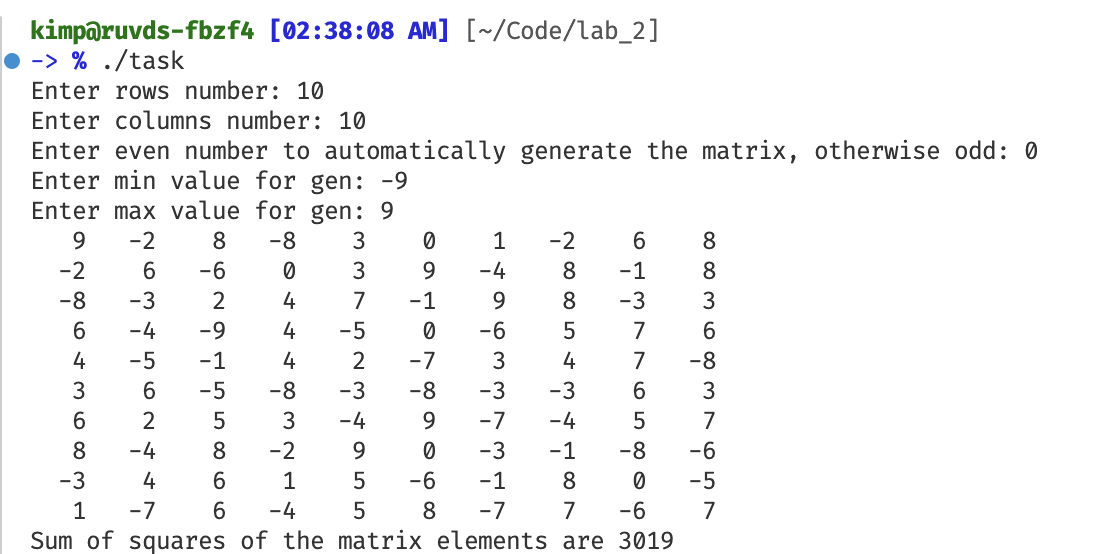
\includegraphics[width=0.7\textwidth]{lab_21.png}
    \caption{Пример работы на марице 10x10 (автогенерация)}
  \end{figure}

  \begin{figure}[H]
    \centering
    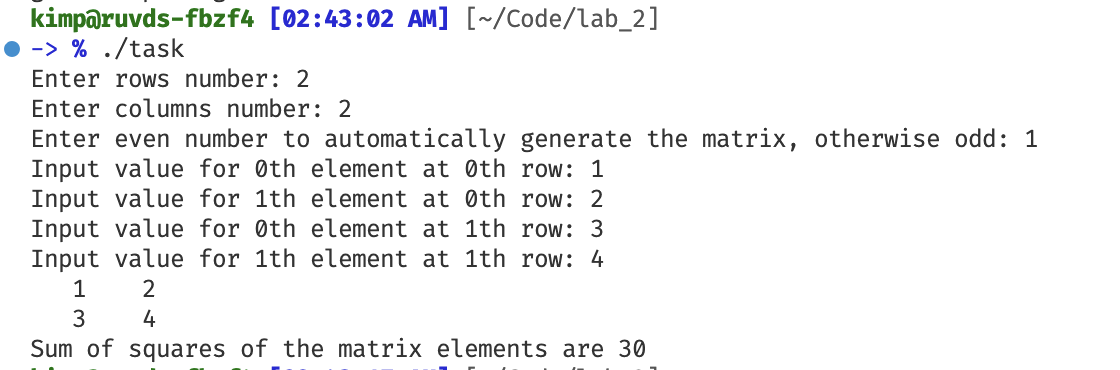
\includegraphics[width=0.7\textwidth]{lab_22.png}
    \caption{Пример работы на марице 2x2 (ручной ввод)}
  \end{figure}

  \begin{figure}[H]
    \centering
    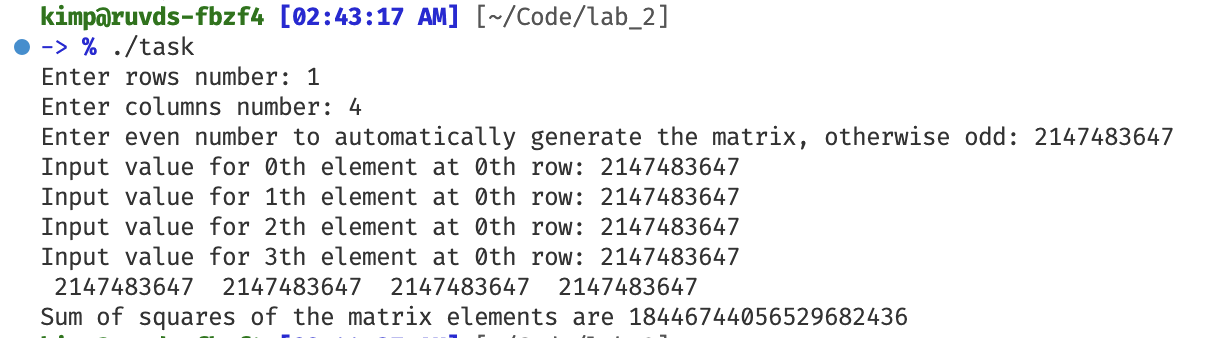
\includegraphics[width=0.7\textwidth]{lab_23.png}
    \caption{Пример работы на марице 1x4 (ручной ввод, без переполнения)}
  \end{figure}

  \begin{figure}[H]
    \centering
    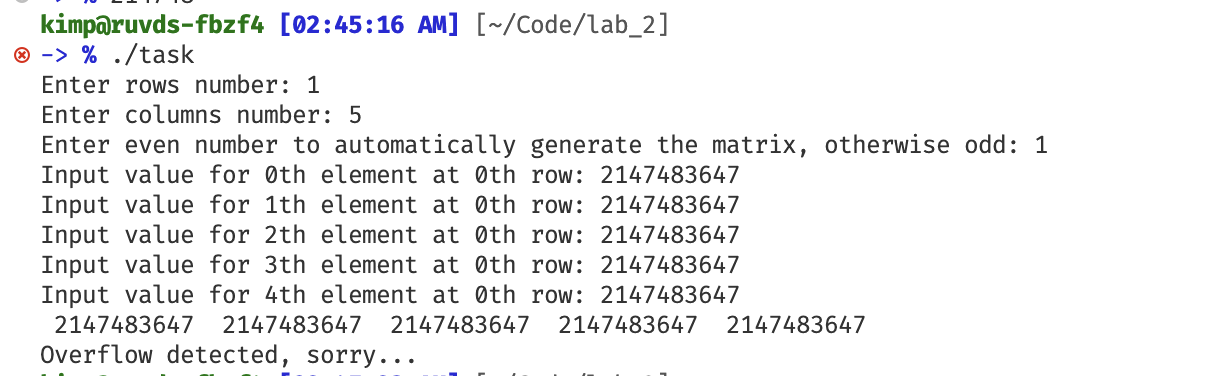
\includegraphics[width=0.7\textwidth]{lab_24.png}
    \caption{Пример работы на марице 1x4 (ручной ввод, с переполнением)}
  \end{figure}
\end{document}
